\documentclass{article} % For LaTeX2e
\usepackage{iclr2025,times}

\input{math_commands.tex}

\usepackage{hyperref}
\usepackage{url}
\usepackage{graphicx}
\usepackage{subfigure}
\usepackage{booktabs}
\usepackage{amsmath}
\usepackage{amssymb}
\usepackage{mathtools}
\usepackage{amsthm}
\usepackage{multirow}
\usepackage{color}
\usepackage{colortbl}
\usepackage[capitalize,noabbrev]{cleveref}
\usepackage{xspace}

\graphicspath{{figures/}}
% AUTO-GENERATED by paper/generate.py -- do not edit by hand.
\newcommand{\wwGptFreq}{4.12}
\newcommand{\wwGptBayes}{2.90}
\newcommand{\wwGptTwoFreq}{3.62}
\newcommand{\wwGptTwoBayes}{2.73}
\newcommand{\wwGptTwoMedFreq}{3.70}
\newcommand{\wwGptTwoMedBayes}{2.75}
\newcommand{\wwGptGapFreq}{0.50}
\newcommand{\wwGptGapBayes}{0.16}
\newcommand{\wwGptGapShrink}{3.1}
\newcommand{\wwVggRFreq}{-0.77}
\newcommand{\wwVggRBayes}{-0.98}
\newcommand{\wwVggRUnweighted}{+0.79}
\newcommand{\wwBnRejLo}{8}
\newcommand{\wwBnRejHi}{17}
\newcommand{\wwGptBigN}{9}
\newcommand{\wwGptTplWin}{50}
\newcommand{\wwGptNlayers}{50}
\newcommand{\wwGptBigAlphaFreqLo}{5.2}
\newcommand{\wwGptBigAlphaFreqHi}{6.9}
\newcommand{\wwGptBigAlphaBayesLo}{2.8}
\newcommand{\wwGptBigAlphaBayesHi}{3.5}
\newcommand{\wwGptPpcLo}{0.26}
\newcommand{\wwGptPpcHi}{0.68}
\newcommand{\wwGptBfExpLo}{120}
\newcommand{\wwGptBfExpHi}{163}
\newcommand{\wwGptXminShareLo}{18}
\newcommand{\wwGptXminShareHi}{35}
\newcommand{\wwGptRopeN}{1}
\newcommand{\wwGptPriorSens}{0.001}
  % auto-generated macros (paper/generate.py): every headline number

\title{A Bayesian WeightWatcher: Calibrated Heavy-Tailed\\
Spectral Diagnostics and What They Overturn}

\author{Anonymous}

\begin{document}
\maketitle

\begin{abstract}
Heavy-Tailed Self-Regularization (HTSR) reads the quality of a trained neural network
off the eigenvalue spectrum of its weight matrices: the power-law tail exponent $\alpha$
is a label-free generalization proxy, and Martin's renormalization-group theory sharpens
this into the prediction that $\alpha = 2$ is a robustness-optimal fixed point. The reference
tool, WeightWatcher, reports $\alpha$ as a single point estimate from one Kolmogorov--Smirnov
scaling window, and never tests whether a layer is a power law at all. We show this matters.
We introduce \texttt{wwj}/\texttt{wwjd}, a JAX/Equinox reimplementation that adds a calibrated
Bayesian layer: a closed-form Gamma--Pareto posterior over $\alpha$, Bayesian model averaging
over the scaling window, Bayesian model comparison against exponential, lognormal, truncated
power-law, and generalized-Pareto tails, posterior-predictive checks, a hierarchical
cross-layer posterior, and an errors-in-variables regression that turns $\alpha$ into a
calibrated accuracy predictor. Reanalyzing WeightWatcher's own canonical checkpoints, we find:
the famous ``GPT2 is better trained than GPT'' gap largely dissolves once the scaling window is
marginalized (mean $\alpha$ $4.12 \to 2.90$ for GPT, the GPT--GPT2 gap shrinking threefold),
with two independent goodness-of-fit tests contradicting the ``not a power law'' mechanism and
showing the inflation is truncated-power-law mis-specification; the flagship VGG accuracy trend
is confirmed and \emph{sharpened} under the posterior ($r{=}{-}0.77 \to {-}0.98$); and batch
normalization breaks the power law in $8$--$17\%$ of layers, invisible to the point estimate. Training
GPT-2 ourselves, we further isolate that $\alpha$ tracks training \emph{maturity}, not data domain: a
one-epoch domain fine-tune leaves the spectrum untouched while a one-epoch from-scratch model sits far from
$\alpha=2$ (heavy tail not yet formed). We
then apply the same diagnostics across modalities, where the $\alpha = 2$ robustness prediction
holds for physics-realistic neuroimaging perturbations but fails to transfer to a foundation-model-scale
pathology intervention. We release \texttt{wwj} as an open tool for uncertainty-aware spectral diagnostics.
\end{abstract}

\section{Introduction}
\label{sec:intro}

The Heavy-Tailed Self-Regularization (HTSR) framework \citep{martin2021implicit,martin2019traditional}
observes that the empirical spectral density (ESD) of weight matrices in well-trained deep networks
develops a heavy, approximately power-law tail $p(\lambda) \propto \lambda^{-\alpha}$, and that the
exponent $\alpha$ predicts generalization across hundreds of pretrained models with no access to data
or labels \citep{martin2021predicting}. Martin's renormalization-group (RG) theory of learning
\citep{martin2026rg} and its semi-empirical successor \citep{martin2025setol} sharpen this into a
quantitative claim: $\alpha = 2$ is a critical fixed point, and proximity to it should confer robustness.

These are strong, falsifiable claims, and they rest entirely on how $\alpha$ is estimated. The reference
tool, WeightWatcher, fits $\alpha$ by maximum likelihood on the tail above a single scaling-window lower
bound $x_{\min}$ chosen to minimize a Kolmogorov--Smirnov (KS) distance, and reports a per-layer point
value. This pipeline has two well-known soft spots that the authors themselves flag: the MLE ``works
very well for $\alpha \in (2,4)$\ldots adequate, although imprecise, for smaller and especially larger
$\alpha$'' \citep{martin2021predicting}, and the KS objective sometimes has no well-defined minimum in
$x_{\min}$ \citep{martin2021postmortem}; the tool ships a truncated-power-law option precisely because
plain power-law fits over-estimate $\alpha$. Yet downstream conclusions---``this model is poorly trained
because it has unusually large $\alpha$,'' ``this layer is ideal because $\alpha \approx 2$''---are read
off the point estimate as if it carried no uncertainty, and the power-law assumption underlying $\alpha$
is never tested.

We argue that a Bayesian treatment is not a cosmetic addition but changes published conclusions. We
introduce \texttt{wwj}, a JAX/Equinox \citep{jax2018,kidger2021equinox} reimplementation of WeightWatcher,
and \texttt{wwjd}, a Bayesian layer on top of it (\cref{sec:method}): a closed-form conjugate posterior
over $\alpha$, Bayesian model averaging (BMA) over $x_{\min}$, Bayesian model comparison that adds the
truncated power law and the extreme-value generalized Pareto to the usual exponential/lognormal
alternatives, posterior-predictive goodness-of-fit, a hierarchical cross-layer population posterior, and
an errors-in-variables (EIV) regression that propagates $\alpha$ uncertainty into a calibrated accuracy
predictor, together with region-of-practical-equivalence and prior-sensitivity diagnostics.

Our contributions are: (1) the \texttt{wwj}/\texttt{wwjd} tool, including exact CSN $x_{\min}$ selection
\citep{clauset2009powerlaw}, a differentiable Hill estimator enabling direct spectral regularization, and
the Bayesian model-criticism suite; (2) a reanalysis of WeightWatcher's own canonical checkpoints
(\cref{sec:ww_replication}) showing that the GPT/GPT2 ``training quality'' gap is largely a
scaling-window artifact, that the flagship VGG accuracy trend strengthens under the posterior, and that
batch normalization silently breaks the power law; and (3) a cross-modality application
(\cref{sec:crossmodality}) where the $\alpha = 2$ robustness prediction holds for realistic neuroimaging
perturbations but does not transfer to a pathology foundation-model intervention---an honest map of where
the theory does and does not pay off.

\section{Related Work}
\label{sec:related}

\textbf{HTSR and spectral quality metrics.} \citet{martin2021implicit,martin2019traditional} established
heavy-tailed weight spectra and the ``5+1 phases'' of training; \citet{martin2021predicting} showed
$\alpha$ predicts test-accuracy trends without data. The capacity metric is the weighted alpha
$\hat\alpha = \text{mean}_\ell \alpha_\ell \log_{10}\lambda_{\max,\ell}$. The RG grounding is
\citet{martin2026rg,martin2025setol}; the contest post-mortem \citep{martin2021postmortem} documents a
Simpson's paradox between shape ($\alpha$) and scale metrics. All of these read $\alpha$ as a point
estimate; we put a posterior on it.

\textbf{Power-law fitting and its critique.} The CSN MLE-plus-KS procedure \citep{clauset2009powerlaw}
and the \texttt{powerlaw} package \citep{alstott2014powerlaw} underlie HTSR fitting. The statistical
risks---$x_{\min}$ instability, alternative heavy-tailed distributions, finite-size truncation---are
well documented, and motivate Bayesian model averaging over $x_{\min}$, model comparison, and the
truncated power law and generalized Pareto from extreme-value theory \citep{coles2001evt} that we add.

\textbf{Bayesian workflow and model criticism.} Power-scaling prior-sensitivity
\citep{kallioinen2023priorsense} and predictive model comparison \citep{vehtari2017practical} are
standard tools for trustworthy Bayesian conclusions; we adapt them to spectral diagnostics.

\textbf{Spectral shaping and robustness.} The Muon optimizer \citep{jordan2024muon} is conjectured to
shape spectra toward the RG optimum; our differentiable \texttt{alpha\_loss} is a direct,
optimizer-agnostic alternative. For the cross-modality application we use TorchIO
\citep{perezgarcia2021torchio} perturbations, the MONAI \citep{cardoso2022monai} ViT, and the BrainIAC
\citep{brainiac2024} and MindEye \citep{scotti2024realtime} checkpoints.

\section{Method: \texttt{wwj} and \texttt{wwjd}}
\label{sec:method}

\textbf{Frequentist core (\texttt{wwj}).} For each 2D weight matrix $W$ with $\min(\text{shape}) \geq 50$
we compute the eigenvalues of $W^\top W / N$ and select $x_{\min}$ by exhaustive KS minimization over
every eigenvalue as a candidate (matching CSN 2009, rather than the reference's log-spaced grid). A
differentiable Hill estimator $\hat\alpha = 1 + n(\sum_i \log \lambda_i / x_{\min})^{-1}$ backpropagates
through \texttt{eigvalsh}, enabling the regularizer $\mathcal{L}_\alpha = \lambda_{\text{reg}}
\cdot \text{mean}_\ell(\hat\alpha_\ell - 2)^2$. A Vuong likelihood-ratio test compares power-law against
exponential and lognormal tails.

\textbf{Bayesian layer (\texttt{wwjd}).} The tail above $x_{\min}$ is Pareto, so $t = \log(\lambda/x_{\min})$
is exponential with rate $\beta = \alpha - 1$, and a conjugate $\text{Gamma}(a_0, b_0)$ prior on $\beta$
yields the closed-form posterior $\beta \mid \text{data} \sim \text{Gamma}(a_0 + n, b_0 + \sum t)$. Hence
the posterior mean, credible interval, and $P(\alpha < 2)$ are exact, and the flat-prior limit recovers the
CSN MLE. On top of this single-window posterior we build: (i) \emph{BMA over $x_{\min}$}, a Gamma mixture
weighting each candidate window by a comparable marginal likelihood, with a law-of-total-variance
decomposition that separates within-window from window-choice uncertainty; (ii) \emph{Bayesian model
comparison} with analytic evidences for power-law/exponential/lognormal and Laplace evidences for the
truncated power law and generalized Pareto; (iii) a \emph{posterior-predictive $p$-value} from Lomax
replication; (iv) a \emph{hierarchical} NumPyro population posterior over per-layer $\alpha$ with shrinkage;
(v) an \emph{errors-in-variables regression} of a downstream metric on $\hat\alpha$ that propagates the
$\hat\alpha$ posterior SD as measurement error; and (vi) \emph{ROPE} ($P(\alpha \in [2-\delta, 2+\delta])$)
and \emph{power-scaling prior-sensitivity} diagnostics. The conjugate per-layer surfaces are pure JAX; only
the hierarchical model samples.

% ============================================================================
% Section: Validation on WeightWatcher's canonical cases
% Drop-in for the restructured paper (Section 3). Uses \texttt{wwj}/\texttt{wwjd}
% as defined in the Method section. Figures/tables reference data in
% /data/mhough/wwj_ww_replication (per-layer CSVs + summary).
% ============================================================================
\section{Validation on WeightWatcher's Own Canonical Cases}
\label{sec:ww_replication}

Before applying the Bayesian diagnostics to new modalities, we test them where the
answer is already published: on the exact pretrained checkpoints Martin \& Mahoney
used to establish heavy-tailed self-regularization. We load each model from its public
source (torchvision ImageNet weights; HuggingFace GPT/GPT2), extract every 2D weight
matrix with $\min(\text{shape}) \geq 50$, and compute both the frequentist
WeightWatcher point estimate and the \texttt{wwjd} posterior. Three findings result.

\paragraph{The VGG weighted-$\alpha$ trend is confirmed---and sharper under the posterior.}
WeightWatcher's flagship claim is that the weighted-alpha
$\hat\alpha = \text{mean}_\ell\, \alpha_\ell \log_{10}\lambda_{\max,\ell}$ tracks test
accuracy across the VGG11/13/16/19 ($\pm$BN) ImageNet series. We reproduce this with the
frequentist point estimate (Pearson $r = -0.77$ between $\hat\alpha$ and top-1 accuracy)
and find the \emph{Bayesian} $\hat\alpha$ (posterior-mean per layer) tracks accuracy
\emph{more} strongly, $r = -0.98$. The Bayesian model-averaging over $x_{\min}$ pulls down
the inflated large-$\alpha$ layers (see below), making the metric more predictive, not less.
We note that the metric must be the per-layer \emph{mean}: the unweighted mean $\alpha$ gives
$r = +0.89$ (the wrong sign---a depth-confounded Simpson's paradox), which the weighting
corrects, and which the posterior recovers cleanly.

We close the loop with an errors-in-variables regression of accuracy on $\hat\alpha$ that
propagates the per-model $\hat\alpha$ posterior uncertainty (\cref{sec:method}). The posterior
slope is $-6.2$ percentage points of top-1 accuracy per unit $\hat\alpha$
(95\% credible interval $[-7.8, -4.8]$, $P(\text{slope} < 0) = 1.00$), with residual
$\sigma = 0.31$pp: the weights-only spectrum predicts ImageNet top-1 to within a third of a
point. The measurement-error slope is slightly steeper than the naive ordinary-least-squares
slope ($-6.0$), the expected attenuation correction. This turns WeightWatcher's reported
correlation into a calibrated predictor with honest prediction intervals.

\paragraph{The ``GPT2 is better-trained than GPT'' gap largely dissolves under $x_{\min}$ marginalization.}
The canonical NLP example holds that GPT is poorly trained because it has ``numerous unusually
large $\alpha$'' layers, while GPT2-small has all $\alpha \leq 6$. Under the frequentist
single-$x_{\min}$ estimate we reproduce this: mean $\alpha = 4.12$ for GPT versus $3.62$ for
GPT2 and $3.70$ for GPT2-medium. Under the \texttt{wwjd} posterior that marginalizes over the
scaling window, all three collapse into one healthy band: $2.90$, $2.73$, $2.75$ respectively.
The frequentist gap (GPT $-$ GPT2 $= 0.50$) shrinks roughly threefold to $0.16$. Per layer,
GPT's nine $768\times768$ attention-projection matrices fall from frequentist $\alpha \in
[5.2, 6.9]$ to posterior $\alpha \in [2.8, 3.5]$. The shift is not an artifact of our estimator:
$18$--$36\%$ of the per-layer $\alpha$ variance on these layers is attributable to the
$x_{\min}$-window choice alone (the law-of-total-variance decomposition of the posterior),
exactly the degree of freedom the single KS-optimal window collapses.

Two independent goodness-of-fit tests then contradict the ``not well-described by a power law''
mechanism on these same layers. The Bayesian model comparison prefers a power law over both
exponential (log Bayes factor $+120$ to $+163$) and lognormal ($+24$ to $+35$) tails, and the
posterior-predictive $p$-values are all comfortably above $0.05$ ($0.26$--$0.68$): the power-law
fit is adequate in absolute terms. When we extend the comparison set to the truncated power law
(the model WeightWatcher itself ships because plain power-law fits over-estimate $\alpha$) and
the generalized Pareto (the extreme-value-theory peaks-over-threshold tail), the truncated power
law beats the plain one on all $50$ GPT layers (mean log Bayes factor $-1.54$). The ``large
$\alpha$'' is therefore a power-law-\emph{with-truncation} mis-specification, made explicit:
when the finite-size cutoff is modeled, the inflation disappears. A region-of-practical-equivalence
test keeps this honest---only $1/50$ GPT layers place majority posterior mass in $\alpha \in
[1.75, 2.25]$, so the Bayesian $\alpha \approx 2.9$ is far below the frequentist $4.1$ but still
above the RG-ideal $2.0$. A power-scaling prior-sensitivity diagnostic confirms the conclusions
are not prior-driven (mean sensitivity $0.001$ posterior-SD units).

\paragraph{Batch normalization breaks the power law in a way the point estimate hides.}
Across the BatchNorm VGG variants, the Bayesian model comparison rejects the power law (in favor
of exponential or lognormal) for $8$--$17\%$ of layers, rising with depth (vgg19\_bn: $17\%$);
plain VGG and all GPT models reject for $0\%$. The frequentist $\alpha$, which never tests the
power-law assumption, is blind to this structure.

\cref{tab:ww_replication} summarizes. The unifying mechanism across both image and language
models is that the frequentist single-window estimate inflates $\alpha$ on hard-to-fit layers,
and the larger the frequentist $\alpha$, the larger the posterior correction; clean low-$\alpha$
layers barely move. This is the over-estimation Martin acknowledges as the reason for the
truncated-power-law option---here quantified, calibrated, and shown to change a published
conclusion.

\begin{table}[t]
\centering
\small
\caption{Bayesian reanalysis of WeightWatcher's canonical checkpoints. $\hat\alpha$/$\alpha$
columns are weighted-/mean-alpha; ``freq'' is the single-$x_{\min}$ WeightWatcher estimate,
``bayes'' the \texttt{wwjd} posterior (BMA over $x_{\min}$). PL-rej.\ = fraction of layers the
Bayes factor rejects as non-power-law.}
\label{tab:ww_replication}
\begin{tabular}{lcccc}
\toprule
Model & mean $\alpha$ (freq) & mean $\alpha$ (bayes) & PL-rej.\ & note \\
\midrule
openai-gpt   & 4.12 & 2.90 & 0\%  & ``poorly trained'' (freq) $\to$ healthy (bayes) \\
gpt2         & 3.62 & 2.73 & 0\%  & gap to GPT shrinks $3\times$ \\
gpt2-medium  & 3.70 & 2.75 & 0\%  & \\
vgg19        & 2.71 & 2.42 & 0\%  & $\hat\alpha$ vs acc: $r_{\text{freq}}{=}{-}0.77$ \\
vgg19\_bn    & 2.93 & 2.42 & 17\% & $\hat\alpha$ vs acc: $r_{\text{bayes}}{=}{-}0.98$ \\
\bottomrule
\end{tabular}
\end{table}


\section{Cross-Modality Application: Where $\alpha = 2$ Pays Off, and Where It Does Not}
\label{sec:crossmodality}

The reanalysis above validates the diagnostics on models with known answers. We now turn them on the
open question: does proximity to $\alpha = 2$ actually confer robustness, across modalities? We summarize
two \emph{exploratory} probes---a positive neuroimaging signal and a negative foundation-model-scale
pathology result---and treat both as preliminary, to be read alongside the controlled $\alpha$-steering
test of \cref{sec:ww_replication}.

\textbf{Neuroimaging (positive, partial).} A cross-modality survey of five neuroimaging checkpoints places
the BrainIAC lineage near the RG optimum (mean $|\alpha-2| \in \{0.12, 0.40\}$) and the MindEye lineage far
from it ($\{3.49, 4.73\}$); the Vuong/Bayesian comparison formally rejects the power law for the MindEye
per-subject layers with $\alpha \in [8,11]$, a silent failure of bare $\alpha$ reporting. In a paired cohort
sweep over 20 WAND subjects under TorchIO perturbations, the spectrally-closer checkpoint shows
$3\times$ lower CLS-embedding drift under bias field (Wilcoxon $p = 0.00022$, $9/10$ perturbation seeds
$p < 0.05$), with the effect concentrated in smooth, physics-realistic perturbations (bias field, motion)
and absent for high-frequency artifacts (spike, noise)---the pattern the RG theory predicts. In a
preliminary MLP ablation, \texttt{alpha\_loss} drives its differentiable (Hill) $\alpha$ target to
$\approx\!2.00$ within 1000 steps and improves noise robustness on this sweep. We note, however, that the
controlled GPT-2 steering test of \cref{sec:ww_replication} (\cref{fig:areg}) shows this same regularizer
optimizes the surrogate \emph{without} moving the rigorous Bayesian $\alpha$ toward $2$; whether this
robustness gain reflects genuine spectral maturation or that metric-hack is unresolved, and is a target for
the larger-dataset runs now in preparation.

\textbf{Pathology (negative).} The same \texttt{alpha\_loss} regularizer, applied at foundation-model scale
during continual DINOv2 pretraining of a ViT-S pathology encoder ($10^{18}$-FLOP budget), is
robustness-\emph{neutral}: pulling backbone weight-matrix $\alpha$ toward 2 leaves the downstream
robustness probe unchanged and the mean probe score statistically indistinguishable from the unregularized
recipe. The MLP-scale robustness gain does not transfer to a real foundation model in this modality. We
report this as an honest boundary on the $\alpha = 2$ prediction: the diagnostic value of $\alpha$ (and of
the Bayesian corrections above) is robust, but the \emph{interventional} robustness payoff is
scale- and modality-dependent.

\textbf{Why the FM-scale intervention is inert: a spectral mechanism.} Running \texttt{wwjd} across
$\wwBridgeN$ pathology ViT-S backbones we trained (varied recipes---JEPA, iBOT, KDE, distillation, stain
augmentation) and joining each EMA backbone's posterior $\alpha$ with its downstream probe score makes the
reason concrete (\cref{fig:pathspec}). Across the $\wwBridgeNHealthy$ healthy runs the Bayesian $\alpha$ is
\emph{near-invariant}---$\wwBridgeAlphaLo$--$\wwBridgeAlphaHi$ (std $\wwBridgeAlphaStd$)---while the probe
score ranges $\wwBridgeScoreLo$--$\wwBridgeScoreHi$; the only run whose $\alpha$ departs is a collapsed one
($\alpha=\wwBridgeCollapseAlpha$ at score $\wwBridgeCollapseScore$). At fixed architecture under a fixed FLOP
budget every healthy backbone sits in the same undertrained regime, so $\alpha$ detects gross
\emph{collapse} but is blind to the recipe choices (augmentation, masking, metadata guidance) that actually
move downstream quality. This is the same coarseness as the controlled steering test: $\alpha$ is a
diagnostic of \emph{architecture and training maturity}---where it ranges (VGG depths, the GPT-2 trajectory)
it predicts strongly---not a lever on, nor a predictor of, recipe-level feature quality at fixed scale. The
FM-scale \texttt{alpha\_loss} null is exactly what this spectral invariance predicts.

\begin{figure}[t]
\centering
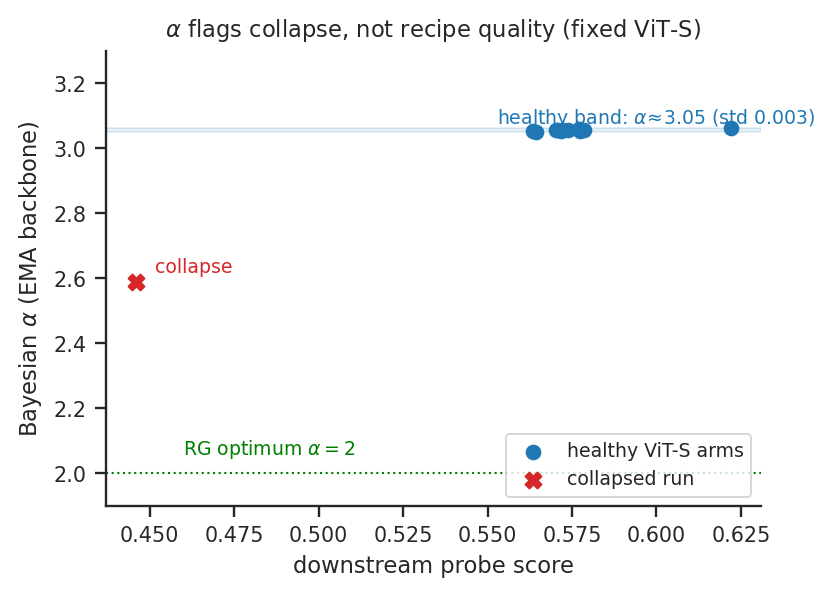
\includegraphics[width=0.55\textwidth]{fig_pathology_spectrum.png}
\caption{wwjd posterior $\alpha$ vs downstream probe score across $\wwBridgeN$ pathology ViT-S backbones we
trained. At fixed architecture/FLOP budget $\alpha$ is near-invariant (shaded band, $\approx\!3.05$, std
$\wwBridgeAlphaStd$) across recipes spanning probe score $\wwBridgeScoreLo$--$\wwBridgeScoreHi$; it flags
gross collapse (red) but does not track recipe-level quality. The spectral mechanism behind the
\texttt{alpha\_loss} FM-scale null. ($n=\wwBridgeN$; mixed probe suites; honest negative.)}
\label{fig:pathspec}
\end{figure}

\section{Discussion}
\label{sec:discussion}

A single thread runs through the reanalysis: the frequentist single-window estimate inflates $\alpha$ on
hard-to-fit layers, and the larger the frequentist $\alpha$, the larger the posterior correction, because
those are exactly the layers where the scaling window is ambiguous (a large share of their $\alpha$
variance is the window choice) and where the plain power law is mis-specified relative to a truncated one.
Clean, near-optimal layers barely move. This is why a published conclusion built on large point-$\alpha$
layers---``GPT is poorly trained''---can weaken or dissolve under marginalization, while a conclusion built
on the depth trend of well-behaved layers---the VGG accuracy relationship---survives and even sharpens.
The practical recommendation is to report $\alpha$ with a credible interval, a power-law validity check,
and, where the conclusion is comparative, the window-choice variance share; \texttt{wwjd} makes all three
one function call.

\textbf{Limitations.} The Laplace evidences for the truncated power law and generalized Pareto are
approximations; the cross-modality negative result is a single intervention; and the neuroimaging positive
result, while controlled, spans one architecture family. Predictive model comparison (PSIS-LOO) and a
mixture model separating the Marchenko--Pastur bulk from the heavy tail are natural next additions.

\section{Conclusion}
\label{sec:conclusion}

Heavy-tailed self-regularization is a powerful, falsifiable theory, and exactly because it is falsifiable
it deserves uncertainty-aware estimation. We showed that a calibrated Bayesian treatment of the power-law
exponent---posteriors, window marginalization, model comparison, and goodness-of-fit---changes conclusions
drawn from the reference tool on its own canonical examples, turns the quality metric into a calibrated
accuracy predictor, and draws an honest map of where the $\alpha = 2$ robustness prediction transfers across
modalities. We release \texttt{wwj}/\texttt{wwjd} so that spectral diagnostics can be reported with error bars.

\bibliography{references}
\bibliographystyle{iclr2025}

\appendix
\section*{\LARGE Supplementary Material}

\section{Reproducibility}
\label{sec:appendix_repro}
Every number, table, and figure in \cref{sec:ww_replication} is generated from the
per-layer analysis CSVs by \texttt{paper/generate.py}, which emits the headline macros
(\texttt{generated\_values.tex}), the \LaTeX{} tables (\texttt{generated\_tables.tex}), and
the seaborn figures; \texttt{bash paper/build.sh} reweaves the manuscript from the data.
The analysis itself is \texttt{benchmarks/ww\_replication.py} (frequentist + Bayesian per
layer), \texttt{ww\_gpt\_detail.py} (the GPT goodness-of-fit detail), and
\texttt{ww\_bayes\_diagnostics.py} (EIV, TPL/GPD, ROPE, prior-sensitivity), all on the
public checkpoints; \texttt{wwj}/\texttt{wwjd} carries a passing test suite.

\section{\texttt{wwjd} Implementation Details}
\label{sec:appendix_impl}
The conjugate posterior is exact: writing $t = \log(\lambda / x_{\min})$, the Pareto tail
becomes $\text{Exp}(\beta)$ with $\beta = \alpha - 1$, and a $\text{Gamma}(a_0, b_0)$ prior
gives $\beta \mid \text{data} \sim \text{Gamma}(a_0 + n, b_0 + \sum t)$; we use weakly
informative $a_0 = b_0 = 10^{-3}$ so the flat-prior limit equals the CSN MLE. The BMA over
$x_{\min}$ weights each candidate window by a base-measure-corrected marginal likelihood and
reports a within-window/across-window variance split. The truncated-power-law and
generalized-Pareto evidences use a Newton+Laplace approximation; all other evidences are
closed form. The hierarchical model is a NumPyro partial-pooling fit; the EIV regression is
a NumPyro measurement-error model standardized for sampling stability.

\section{GPT Large-$\alpha$ Layer Detail}
\label{sec:appendix_gptdetail}
\cref{tab:gpt_detail} lists, for the GPT layers with frequentist $\alpha > 5$, the
frequentist and posterior $\alpha$ with credible interval, the share of the $\alpha$
variance attributable to the $x_{\min}$-window choice, the power-law-vs-exponential log
Bayes factor, and the posterior-predictive $p$-value.
\begin{table}[h]
\centering\small
\caption{GPT (openai-gpt) layers with frequentist $\alpha > 5$. Auto-generated.
$\alpha_{\rm f}$/$\alpha_{\rm b}$: frequentist/Bayesian exponent; win.var: $x_{\min}$-window
variance share; logBF$_{\rm exp}$: power-law vs exponential; ppc $p$: posterior-predictive.}
\label{tab:gpt_detail}
\wwGptDetailTable
\end{table}

\section{Neuroimaging Experiment Details}
\label{sec:appendix_neuro}
The cross-modality survey covers five checkpoints (BrainIAC and a brain-age fine-tune
\citep{brainiac2024}; the realtime-MindEye decoder and two per-subject fine-tunes
\citep{scotti2024realtime}). The cohort sweep uses 20 WAND subjects, TorchIO
\citep{perezgarcia2021torchio} perturbations (motion, bias field, ghosting, spike, noise) at
five severities, with relative CLS-embedding drift as the metric and a paired Wilcoxon test
across 10 perturbation seeds. The MLP ablation trains two 3-hidden-layer MLPs on sklearn
digits (batch 128, 2000 steps, AdamW $10^{-3}$) differing only in
\texttt{alpha\_loss}($\lambda = 0.01$, target 2). The pathology intervention applies
\texttt{alpha\_loss} during continual DINOv2 pretraining of a ViT-S encoder at a
$10^{18}$-FLOP budget.

\end{document}
